\chapter{Konzeption des Generative Adversarial Networks}
\ac{GTSRB}
\begin{figure}[H]
   \centering
   \begin{subfigure}[b]{0.2\textwidth}
       \centering
       
\includegraphics[height=\textwidth]{../images/GTSRB/00093.png}
       \caption{}
       \label{fig:gtrsb-paper-bsp-image-1}
   \end{subfigure}
   \hspace{2em}%
   \begin{subfigure}[b]{0.2\textwidth}
       \centering
       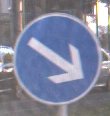
\includegraphics[height=\textwidth]{../images/GTSRB/00847.png}
       \caption{}
       \label{fig:gtrsb-paper-bsp-image-2}
   \end{subfigure}
   \hspace{2em}%
   \begin{subfigure}[b]{0.2\textwidth}
       \centering
       
\includegraphics[height=\textwidth]{../images/GTSRB/00040.png}
       \caption{}
       \label{fig:gtrsb-paper-bsp-image-3}
   \end{subfigure}
   \hspace{2em}%
   \begin{subfigure}[b]{0.2\textwidth}
    \centering
    
\includegraphics[height=\textwidth]{../images/GTSRB/00052.png}
    \caption{}
    \label{fig:gtrsb-paper-bsp-image-4}
\end{subfigure}
      \caption{Beispielbilder aus dem \acs{GTSRB} Datensatz \cite{GTSRB}}
      \label{fig:gtrsb-paper-bsp-images}
\end{figure}
\cite{GTSRB}
\section{Datensatz}
\section{Framework}
\section{Architektur}
\section{Datenaugmentation}
\section{Training}